Với sự phát triển của EA các nhà nghiên cứu đã và đang tiếp tục đưa ra những hướng nghiên cứu mới, những thuật toán hiệu quả cao hơn. Trong những năm gần đây, \emph{tiến hóa đa nhiệm} nổi lên như là một xu hướng trong cộng đồng các nhà nghiên cứu \emph{thuật toán tiến hóa} và \emph{tính toán thông minh}. Không chỉ một mà nhiều bài toán tối ưu có thể được giải quyết cùng nhau, điều này còn được gọi với cái tên khác là \emph{tối ưu hóa đa tác vụ} (thuật ngữ gốc: \emph{multitask  optimization}.

Trong khoa học máy tính và học máy có một thuật ngữ được gọi là \emph{học đa nhiệm vụ } (thuật ngữ gốc: \emph{multitask learning}) nó khá tương đồng với \emph{multitask  optimization}. Trong \textbf{multitask learning} các tác vụ liên quan sẽ chia sẻ kiến thức với nhau, và được huấn luyện cách đồng thời. Lấy ví dụ trong hệ thống phân loại email rác, có thể coi đây là các tác vụ phân loại riêng biệt nhưng có liên quan giữa các người dùng với nhau. Cụ thể hơn, những người khác nhau sẽ có những cơ chế, đặc tính phân loại tin email và email thường khác nhau. Tuy nhiên, hầu hết người dùng đều không tự gán nhãn đủ để có thể xây dựng cơ chế đủ tốt phân loại email cá nhân hóa, trong khi dữ liệu lại quá nhiễu để sử dụng cơ chế phân loại chung cho tất cả các người dùng. Bởi vậy kỹ thuật \textbf{multitask learning} sẽ dựa vào thông tin từ những người dùng thường xuyên gán nhãn email để làm cơ sở kiến thức trong việc xây dựng cơ chế cá nhân hóa cho các người dùng khác. Trong khi đó, \textbf{multitask  optimization} cũng giúp các tác vụ được tối ưu một cách đồng thời nhưng là một thuật ngữ chung hơn, nó không phụ thuộc vào việc các thông tin trong mô hình được kết nối với nhau như thế nào để chia sẻ. Mà nó giúp giữa các tác vụ có liên quan đến nhau có thể chia sẻ không gian giải pháp với tác vụ khác để đẩy tốc độ tìm kiếm giải pháp tối ưu trên tác vụ đó, bao gồm cả các giải pháp rời rạc và tối ưu. 

Để cụ thể hơn, lấy ví dụ bài toán \emph{dịch vụ đám mây theo yêu cầu} (thuật ngữ gốc: \emph{cloud-based-on-demand}) cung cấp cho khách hàng sử dụng. Có thể hiểu là hệ thống sẽ phải giải quyết nhiều tác vụ tối ưu cùng lúc được nhận từ nhiều người dùng vào cùng một thời điểm. Mỗi tác vụ có thể có những đặc tính chung nào đó hoặc chúng hoàn toàn khác nhau. Nói một cách khác \textbf{multitask optimization} có thể được xem như là một mô thức chung trong việc giải quyết các bài toán tối ưu hóa. Không chỉ là việc chia sẻ kiến thức 1 chiều từ những tác vụ đơn giản đến tác vụ phức tạp, mà thực tế khi giải quyết những tác vụ phức tạp sẽ có thể giải quyết được những tác vụ đơn giản hơn. 

Một cách tiếp cận \empth{tiến hóa} cho \empth{multitask optimization} được gọi là \empth{evolutionary multitasking} hay còn gọi là tiến hóa đa tác vụ. Nó là một phương pháp kết hợp tư tưởng của thuật toán EA theo hướng tối ưu hóa nhiều vấn đề một cách đồng thời dựa theo cơ sở của lý thuyết \empth{multitask optimization}.
% \begin{figure}[ht]
%     \centering
%     \fbox{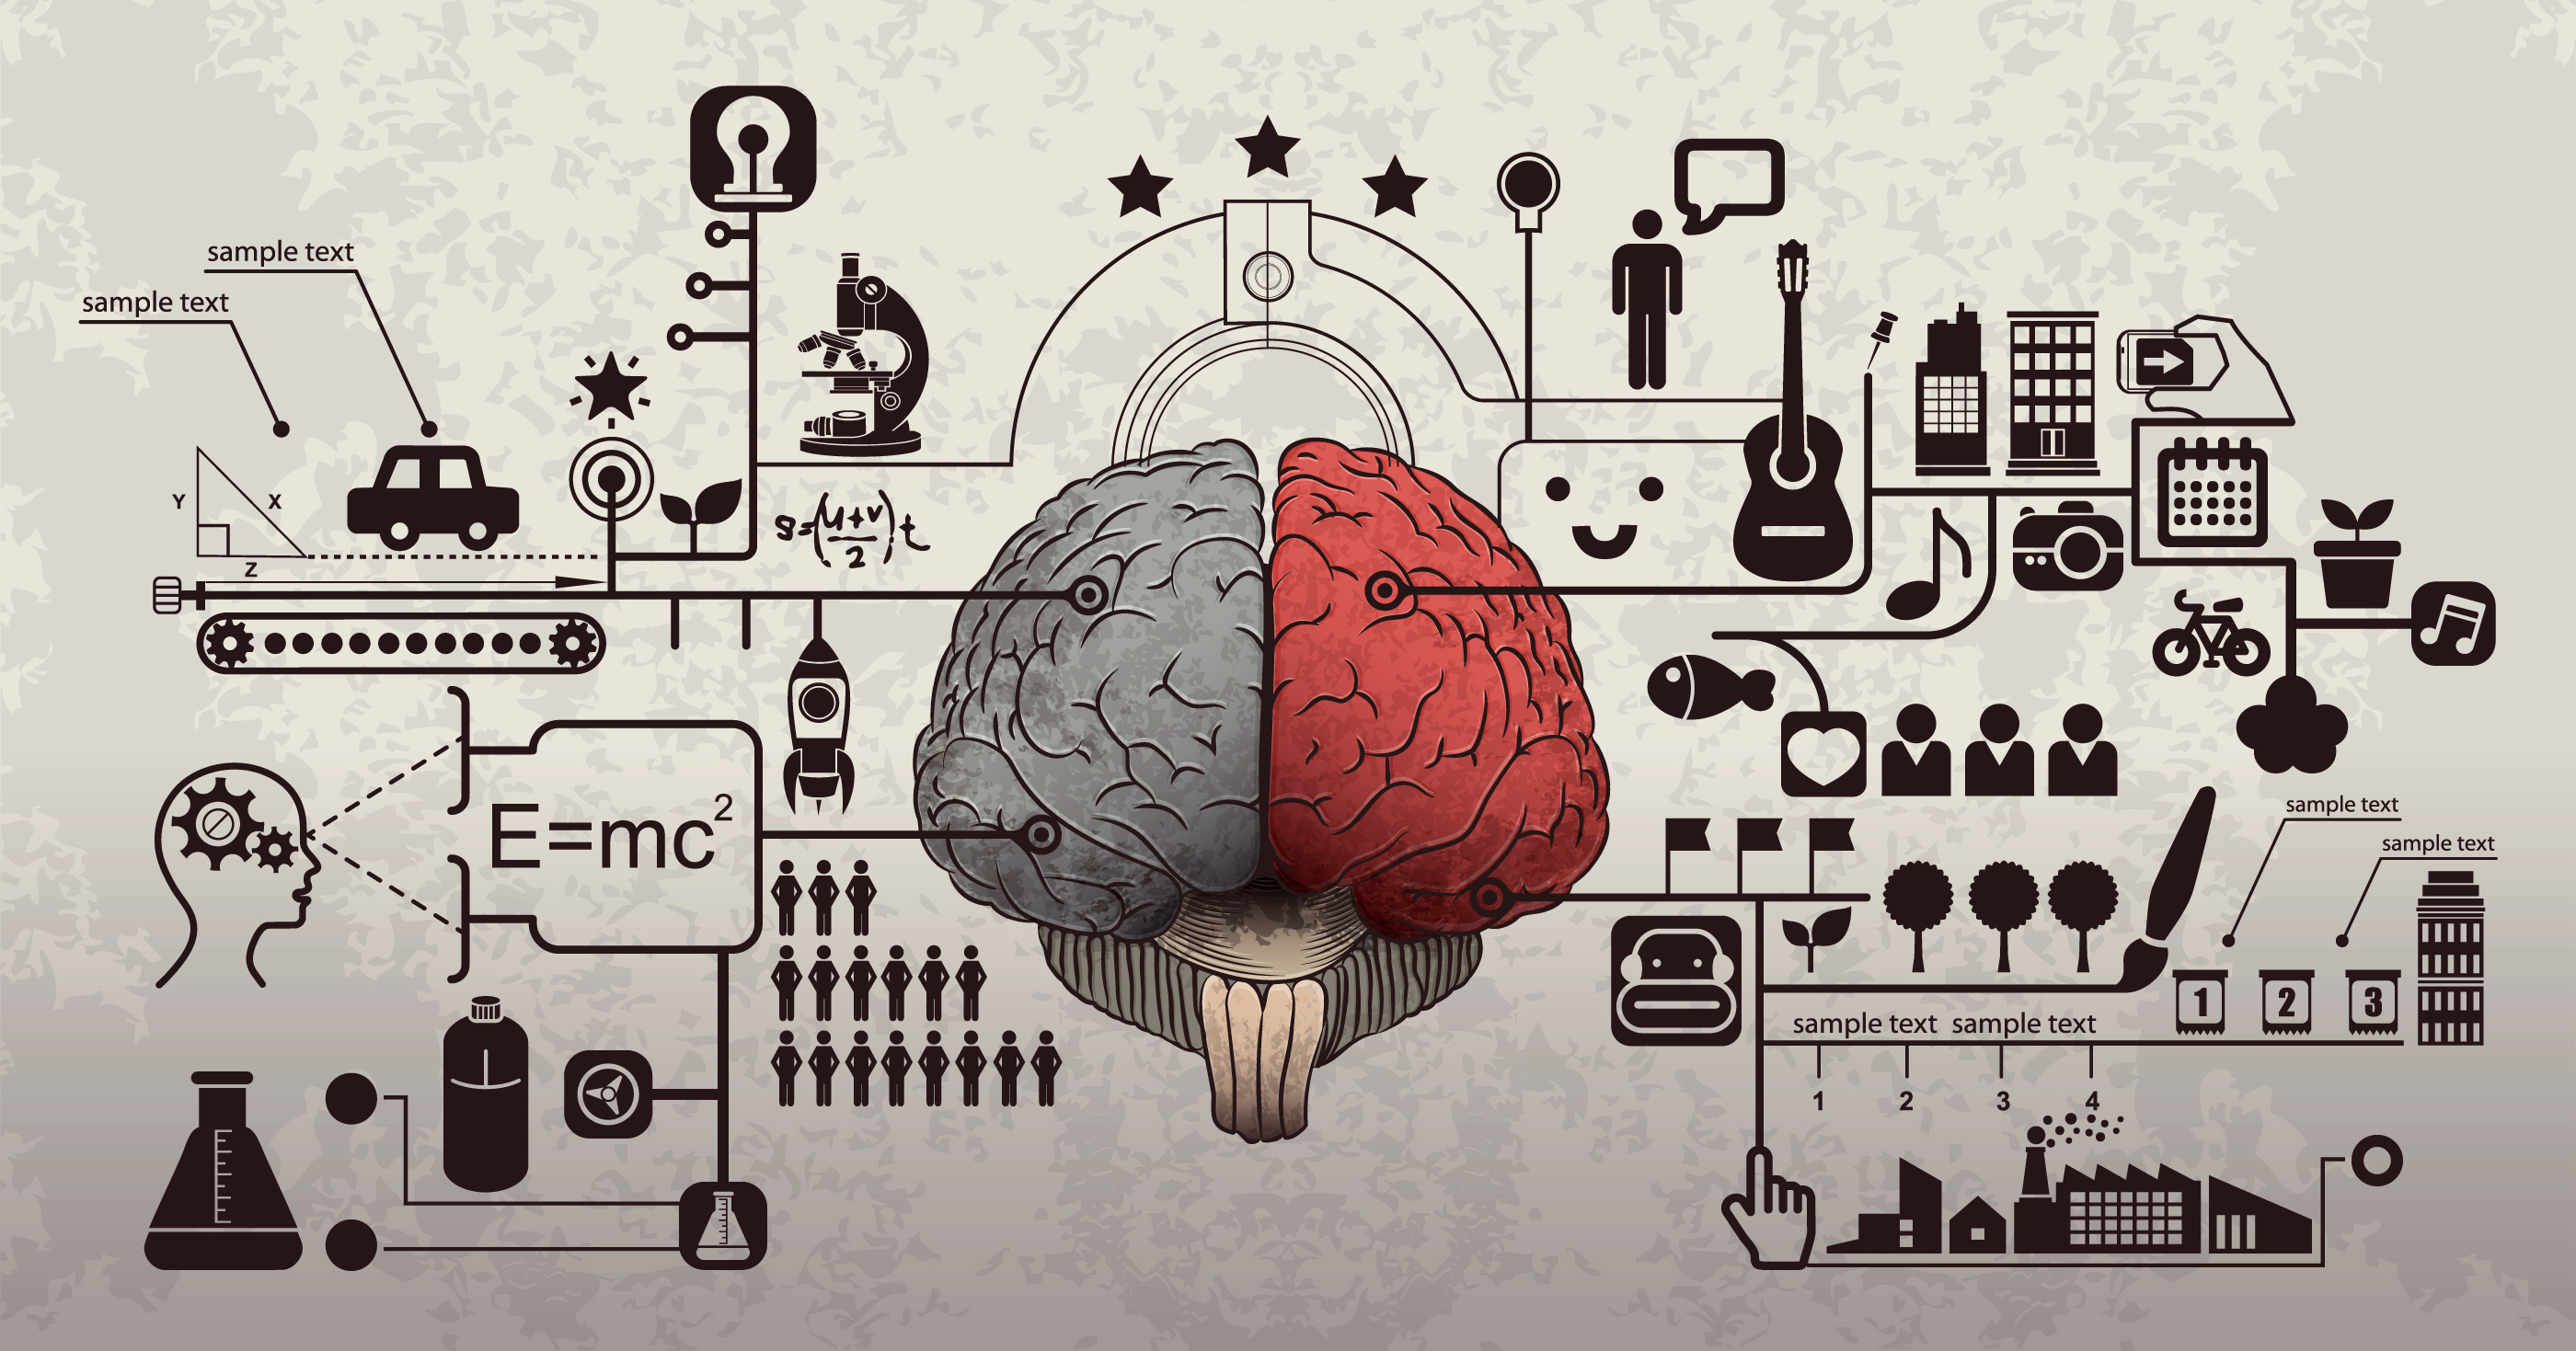
\includegraphics[width=0.6\linewidth]{mindfulness.jpg}}
%     \caption{Mô tả về đa nhiệm của nhận thức khi bộ não liên tục phải nhận nhiều tín hiệu từ các nguồn khác nhau và xử lý chúng đồng thời}
%     \label{fig:mfea:cognitive-multitasking}
% \end{figure}

Bên cạnh đó, tiến hóa đa nhiệm còn lấy cảm hứng ý tưởng từ tưởng, não của con người có thể giải quyết được nhiều tác vụ cùng một lúc. Lấy ví dụ, con người thường hay nói chuyện khi đi bộ, nghe nhạc khi đang học, vừa hát vừa đánh đàn vv.. các công việc này đều yêu cầu não bộ phải xử lý các thông tin khác nhau từ các tác vụ khác nhau. Một đứa trẻ khi lớn lên đã phải có khả năng giải quyết nhiều việc cùng một lúc, học nhiều môn học, học nhiều thứ tiếng. Việc giải quyết nhiều tác vụ cùng một lúc giờ đây là điều tất nhiên con người phải thích nghi để sống sót, tồn tại trong xã hội. So với trước đây, não bộ con người ngày càng được yêu cầu cao hơn, đòi hỏi phải xử lý nhiều thông tin hơn. Có một điểm cần lưu ý là tuy não bộ con người giải quyết nhiều tác vụ cùng một lúc, tuy nhiên khi chuyển từ tác vụ này sang tác vụ khác, nó có khả năng tái sử dụng những kinh nghiệm đã học được từ tác vụ trước đó để giải quyết tác vụ tiếp theo. 